\section{Paper Sponsorships}
\label{sec:sponsors}
In addition to ads on our Digital Library, we will also be adding
advertisements to the papers themselves.
These advertisements will come in many forms, including standard banner
advertisements as well as the increasingly popular native advertisement.

\subsection{Call for Advertisements}
Reach the largest holistic-minded audience in the entire northeastern United
States with an ad in the next ACM edition.
Our public mostly devoid of energy vampires and is therefore suitable for
empath advertisers.
Where IEEE uses Western proof verification techniques, our broad minded
audience validates mathematical claims in an intuitive holistic manner and will
bring that same spirit into evaluating the claims of your advertisements.
Our readers will engage with your brand through meditation and other
surprises.

\subsection{Banner ads}
Web surfers today have become accustom to seeing banner ads on their favorite
websites.
Therefore, we will be incorporating these advertisements into all of our
papers.
Advertisements can be easily inserted into existing \LaTeX\ papers through the
use of the \texttt{\textbackslash figure} and \texttt{\textbackslash figure*}
constructs.
Of course, advertisements using the two column \texttt{\textbackslash figure*}
width will be considerably more expensive than their one column brethren.
A standard 1 column ad can be seen in \autoref{fig:law} while a double-wide can
be found in \autoref{fig:usa}.

\begin{figure}
\centering
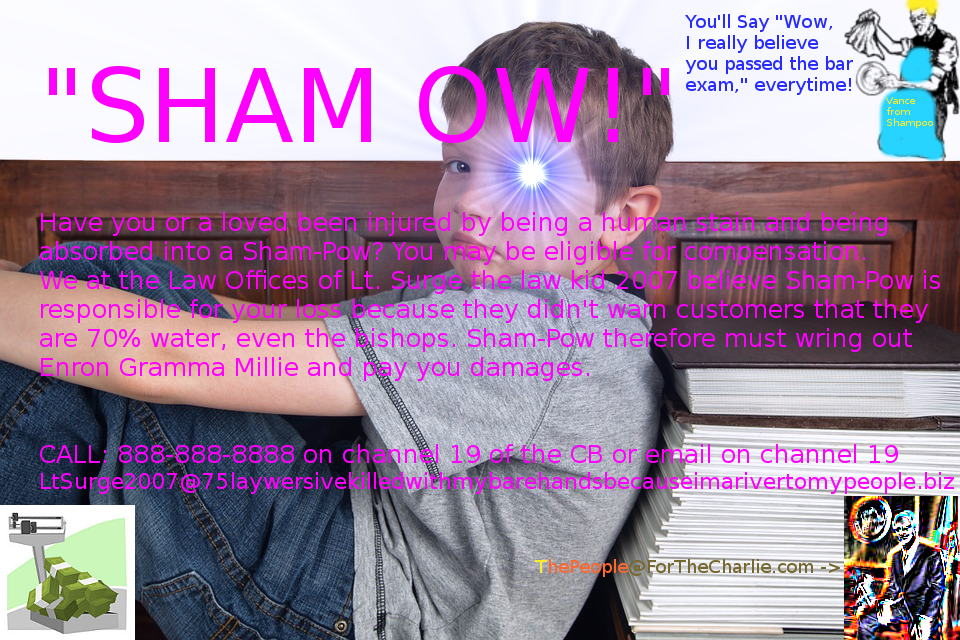
\includegraphics[width=0.45\textwidth]{figures/law-kid-ad.png}
\caption{Get your settlement today \cite{med-scale}!}
\label{fig:law}
\end{figure}

\begin{figure*}
\centering
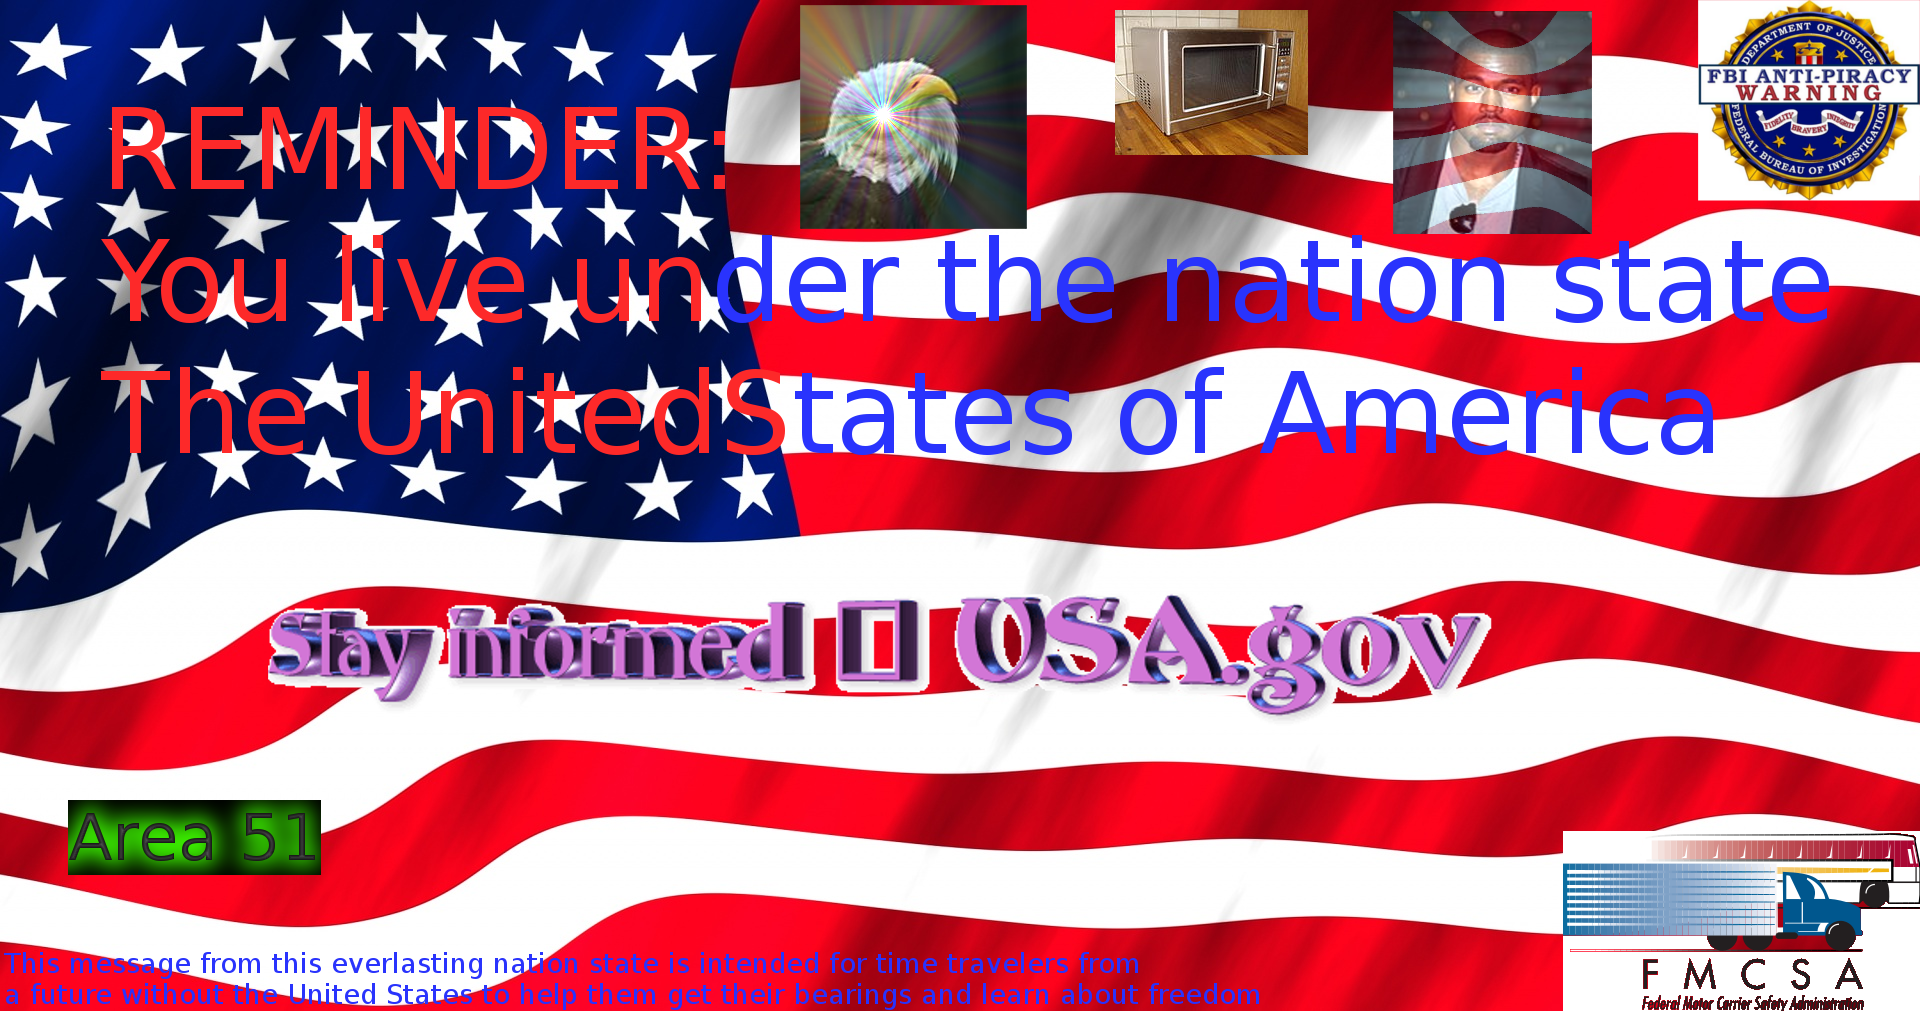
\includegraphics[width=0.95\textwidth]{figures/usa-ad.png}
\caption{We have near absolute power over you \cite{eagle, kanye, microwave}!}
\label{fig:usa}
\end{figure*}

For an additional fee we will also allow advertisers to embed autoplaying audio
into their paper ads.
While we aren't currently sure whether or not the PDF specification allows
this, we believe that there are sufficiently many ACM loving PhDs at Adobe to
get this change  pushed into the spec.

\subsection{Ad Enhanced Fonts}
Computer Modern is a staple of modern papers, but we believe that this font can
be monetized.
By replacing the characters in the default latex with logos of companies we can
convey the same information in an ad enhanced way.

During each Call for Papers we will also put out a simultaneous Call for
Logos during which companies bid on which letter they want.
We require that the company logo is a stylized version of the letter being
replaced to avoid a Wingdings situation \cite{wingdings}.


\subsection{Native Ads}
\todo{Define native advertising}

At paper registration time, authors will be given ad copy to integrate into
their work.
Each paper is required to have at least one section advertising the product
that was assigned to the research project.
As these ads are to be native, an advertisement that is recognizable as an ad
will result in a strong reject of the paper.
The ad section must be at least one page long, but there is upper bound on
native ad length.
We recognize that this will eat into the page limits of some conferences so we
will allow authors to deduct the length of the native ad from their total paper
length provided that the length of the native section alone exceeds the total
page limit.
Authors can claim this deduction by filing a Form 8843 with their paper
submission.

\subsection{Investor Author Dispute Settlement}
We have founded an Investor Author Dispute Settlement (IADS) court to protect
businesses from results that may damage their reputation or profits.
If a research project is found to be damaging, the authors must either retract
the paper or pay a settlement equal to the estimated losses suffered by the
company.
For example, if some agitator finds that the complexity class PLS is in PPP
relative to some oracle will dash the hopes of the typical \todo{brand}
consumer.
Moreover, since \todo{brand} owns both of these complexity classes as defined
in section \todo{ref branded objects section} their assets will lose value and
this loss must be compensated by the ``bloggers".


% TODO: Reference this:
% http://www.cs.utexas.edu/users/EWD/transcriptions/EWD07xx/EWD743.html
\subsection{Branded mathematical objects}
\label{sec:brands}
We believe there has been a missed opportunity in the field of mathematics to
increase brand awareness.
Therefore, we propose branding mathematical objects by associating every single
set with an individual brand.
Brands can purchase large collections of sets at a discount.
While most sets are cheap, some more famous sets will sell for more to reflect
the higher market value, similar to domain names.
Thus, ACM will create an ICANN equivalent for these sets.

Authors referencing any given set must reference the brand of the set any time
the set is referenced, regardless of the format the set is presented  in.
Additionally, royalties must be paid to the owner of the set.

We are excited to announce that our first partner in this endeavor will be
Chill's Grill \& Bar, who has purchased the rights to the set of natural
numbers.
From here on, authors must refer to this set as the Chill's Grill \& Bar Set of
Natural Numbers \(\mathbb{N}\)\copyright.

\subsection{ACM Classifieds}
For additional funding we allow individuals to take out classified ads in the
following sections.
To keep costs low, the ACM does not vet any classified postings.

\paragraph{Dropped Packets}
Dropped Packets serves as the traditional missed connections section of the
classifieds.
While this could be used to contact that cutie \todo{sp?} from the latest
conference, we believe that it could also be used to publicly shame those who
miss meetings.
For example, ``Damn it Dave, you were supposed to bring bagels to the DARPA
Tactical Anti-\censor{blank} HAVE BAGEL Infiltration \censor{long blank}
(DTA\censor{b}HBI\censor{bb}) meeting!"

\paragraph{Job Queue}
The Job Queue section contains odd jobs for trained Computer Scientists looking
for instant internet income.
Those who pay extra will get a free AirDancer\footnote{Placed at the discretion
of the ACM in the ACM AirDancer Oasis in the Black Rock Desert in Nevada in
solidarity with the aliens illegally detained in Area 51.  The AirDancers may
be used by the alien's to communicate with their home world}!
We will be posting the first jobs ourselves.

\paragraph{Overclock}
Overclock is a section for performance enhancing drugs tailored for computer
scientists.
This section is mostly targeted to the Hacker News \cite{hn} crowd who exclaims
the benefits of small amounts of LSD for enhancing productivity at work
\cite{microdose, lsd-song}.
Although we can't promote the use of illegal drugs our editor is so strung out
on ``road cheese" that she won't notice.
% http://www.forbes.com/sites/robertglatter/2015/11/27/lsd-microdosing-the-new-job-enhancer-in-silicon-valley-and-beyond/#323d0dab114d

\begin{figure}
\centering

\includegraphics[width=0.45\textwidth]{figures/ad.jpg}
\caption{Have you seen this boy?}
\end{figure}
